\section{BGK, AWBS, and Fokker-Planck models in local diffusive regime}
\label{sec:DiffusiveKinetics}

We can try to find an~approximate solution while using the~first term of
expansion in $\mfpei$ and $\mu$ as
\begin{equation}
  \tilde{f}(z, \vmag, \mu) = f^0(z, \vmag) + f^1(z, \vmag) \mfpei\mu ,
  \label{eq:f_approximation}
\end{equation}
where $\mfpei = \frac{\vmag}{\nuei} = \frac{\vmag^4}{\Zbar n_e \Gamma}$.

\begin{multline}
  \mu\left(\pdv{\tilde{f}}{z} + \frac{\tEz}{\vmag}\pdv{\tilde{f}}{\vmag}\right) 
  + \frac{\tEz(1-\mu^2)}{\vmag^2}\pdv{\tilde{f}}{\mu} = \\
  \mu\left(\pdv{f^0}{z} + \frac{\tEz}{\vmag}\pdv{f^0}{\vmag}\right) 
  + \frac{\tEz\mfpei}{\vmag^2} f^1 + O(\mu^2) ,
  \nonumber
\end{multline}

\subsection{The~BGK local diffusive electron transport}
\label{sec:BGKDiffusiveRegime}

\begin{equation}
  \frac{1}{\vmag}C_{BGK}(f)
  =
  \frac{f - \fM}{\mfpe}
  + \frac{1}{2 \mfpei}
  \pdv{}{\mu}(1 - \mu^2)\pdv{f}{\mu} ,
  \label{eq:OOE_AWBS_model_1D}
\end{equation}

\begin{eqnarray}
  f^0 &=& \fM + \frac{\tEz}{\vmag^2}f^1 \Zbar\mfpei^2 ,
  \label{eq:BGK_f0} \\
  f^1 &=& - \frac{\Zbar}{\Zbar+1}
  \left( \pdv{f^0}{z} + \frac{\tilde{E}_z}{\vmag}\pdv{f^0}{\vmag} \right) , 
  \label{eq:BGK_f1}
\end{eqnarray}
%\begin{equation}
%  \tilde{f} = \fM - \frac{\Zbar}{\Zbar+1}
%  \left(\frac{1}{\rho}\pdv{\rho}{z} + 
%  \left( \frac{\vmag^2}{2 \vth^2} - \frac{3}{2}\right)
%  \frac{1}{T}\pdv{T}{z} - \frac{\tilde{E}_z}{\vth^2} \right)\fM \mfpei \mu , 
%  \nonumber
%\end{equation}
and when holds 
\begin{multline}
\vect{j} \equiv \qe \int \vv f^1 \, \dI\vv = \vect{0}  \rightarrow
\tE = \vth^2\left(\frac{\nabla\rho}{\rho} + \frac{5}{2}\frac{\nabla T}{T} 
\right) ,
\nonumber
\end{multline}
i.e. the~electric field $\tEz$ obeying the~zero current condition leads to
\begin{equation}
  \tilde{f} = \fM - \frac{\Zbar}{\Zbar+1}
  \left( \frac{\vmag^2}{2 \vth^2} - 4\right)
  \frac{1}{T}\pdv{T}{z}\fM \mfpei \mu , 
  \nonumber
\end{equation}

\subsection{The~AWBS diffusive electron transport}
\label{sec:AWBSDiffusiveRegime}

\begin{multline}
  \frac{1}{\vmag}C_{AWBS}(f)
  = 
  \frac{\vmag}{2\mfpe} \pdv{}{\vmag}\left(f - \fM\right) \\
  + \frac{1}{2}\left(\frac{1}{\mfpei} + \frac{1}{2\mfpe}\right)
  \pdv{}{\mu}(1 - \mu^2)\pdv{f}{\mu} ,
  \label{eq:OOE_AWBS_model_1D}
\end{multline}

\begin{eqnarray}
  \pdv{}{\vmag}\left( f^0 -\fM\right) &=& 
  \frac{\tEz}{\vmag^3}f^1 2\Zbar\mfpei^2 ,
  \label{eq:AWBS_f0} \\
  \frac{\vmag}{2\Zbar\mfpei}\pdv{\left(f^1 \mfpei\right)}{\vmag}  
  - \frac{2\Zbar + 1}{2\Zbar} f^1 &=&
  \pdv{f^0}{z} + \frac{\tilde{E}_z}{\vmag}\pdv{f^0}{\vmag}
  \nonumber 
  %\\  
  %\frac{\vmag}{\Zbar}\pdv{f^1}{\vmag} + \frac{4}{\Zbar}f^1 
  %- \frac{\Zbar + 1}{\Zbar} f^1 &=&
  %\pdv{f^0}{z} + \frac{\tilde{E}_z}{\vmag}\pdv{f^0}{\vmag}
  %\nonumber
\end{eqnarray}

\begin{multline}
  \pdv{f^1}{\vmag} + \frac{1}{\vmag}(3-2\Zbar)f^1
  = \\
  \frac{2\Zbar}{\vmag}\left(\frac{1}{\rho}\pdv{\rho}{z} + 
  \left( \frac{\vmag^2}{2 \vth^2} - \frac{3}{2}\right)
  \frac{1}{T}\pdv{T}{z} - \frac{\tilde{E}_z}{\vth^2}\right)\fM .
  \label{eq:AWBS_f1}
\end{multline}

\subsection{The~Fokker-Planck diffusive electron transport}
\label{sec:FPDiffusiveRegime}
\newcommand{\gt}{g}
\newcommand{\gM}{\gt_M}

The~Fokker-Plank collision operator can be written as 
\cite{Shkarofsky_Particle_Kinetics_book_1966_24}
\begin{equation}
  \frac{1}{\vmag}C_{FP}(f) =  
  \frac{\Gamma}{\vmag} \left(4\pi f^2 
  + \frac{\gv\gv \ft : \gv\gv \gt}{2}\right) ,
  \nonumber
\end{equation}
where $g(\vv) = \int |\vv - \vvb| f(\vvb)\, \dI\vvb$ is 
the~Rosenbluth potential \cite{Rosenbluth_PR1957}. Since we are interested in 
the~approximate solution in the~diffusive regime, it is convenient to
use a~low anisotropy approximation 
$\tilde{\gt} = \gt^0(f^0) + \gt^1(f^1) \mfpei \mu$, which arises from 
Eq. 45 in \cite{Rosenbluth_PR1957}.

\begin{multline}
  C_{FP}(\tilde{f}) = 
  \Gamma\left(4\pi{\ft^0}^2 + 
  \frac{1}{2}\frac{\partial^2 \ft^0}{\partial \vmag^2}
  \frac{\partial^2 \gt^0}{\partial \vmag^2}
  + \frac{1}{\vmag^2}\pdv{\ft^0}{\vmag}\pdv{\gt^0}{\vmag} \right)
  \\
  + \frac{\mu}{\Zbar n_e}
  \Bigg[8\pi \ft^0 \ft^1\vmag^4 - \vmag\left(\pdv{\ft^0}{\vmag}\gt^1
  + \pdv{\gt^0}{\vmag}\ft^1\right) 
  \\
  + \frac{1}{\vmag^2}\left(\pdv{\ft^0}{\vmag}
  \pdv{(\gt^1\vmag^4)}{\vmag}
  + \pdv{\gt^0}{\vmag}\pdv{(\ft^1\vmag^4)}{\vmag}\right) \\
  + \frac{1}{2}\left(\frac{\partial^2 \ft^0}{\partial \vmag^2}
  \frac{\partial^2 (\gt^1\vmag^4)}{\partial \vmag^2}
  + \frac{\partial^2 \gt^0}{\partial \vmag^2} 
  \frac{\partial^2 (\ft^1\vmag^4)}{\partial \vmag^2}
  \right) \Bigg] + O(\mfpei^2, \mu^2) ,
  \nonumber
\end{multline}
where the~isotropic contribution $O(\mfpei^2) = \frac{2}{\vmag^2}
  \left(\pdv{\ft^1\mfpei}{\vmag} - \frac{\ft^1\mfpei}{\vmag} \right)
  \left(\pdv{\gt^1\mfpei}{\vmag} - \frac{\gt^1\mfpei}{\vmag} \right)$.

\begin{multline}
  4\pi{\ft^0}^2 + 
  \frac{1}{2}\frac{\partial^2 \ft^0}{\partial \vmag^2}
  \frac{\partial^2 \gt^0}{\partial \vmag^2}
  + \frac{1}{\vmag^2}\pdv{\ft^0}{\vmag}\pdv{\gt^0}{\vmag} = 
  \frac{\tEz}{\vmag^5}f^1 \Zbar n_e\mfpei^2 \\
  - \frac{2}{\vmag^2}
  \left(\pdv{\ft^1\mfpei}{\vmag} - \frac{\ft^1\mfpei}{\vmag} \right)
  \left(\pdv{\gt^1\mfpei}{\vmag} - \frac{\gt^1\mfpei}{\vmag} \right),
  \label{eq:FP_f0} 
\end{multline}
where the~fundamental property of the~Fokker-Planck collision operator
is to tend to Maxwell-Boltzmann distribution \cite{Longmire_1963}, i.e.
$f^0 = \fM$.
%\begin{multline}
%  \frac{1}{2}\left(\frac{\partial^2 \ft^0}{\partial \vmag^2}
%  \frac{\partial^2 (\gt^1\vmag^4)}{\partial \vmag^2}
%  + \frac{\partial^2 \gt^0}{\partial \vmag^2} 
%  \frac{\partial^2 (\ft^1\vmag^4)}{\partial \vmag^2}
%  \right) 
%  + \frac{1}{\vmag^2}\left(\pdv{\ft^0}{\vmag} \pdv{(\gt^1\vmag^4)}{\vmag} 
%  + \pdv{\gt^0}{\vmag}\pdv{(\ft^1\vmag^4)}{\vmag}\right) \\
%  - \vmag\left(\pdv{\ft^0}{\vmag}\gt^1 
%  + \pdv{\gt^0}{\vmag}\ft^1\right)
%  + 8\pi \ft^0 \ft^1\vmag^4 
%  - \vmag \ft^1
%  = 
%  \vmag\pdv{f^0}{z} + \tilde{E}_z\pdv{f^0}{\vmag}
%  ,
%  \label{eq:FP_f1}
%\end{multline}

\begin{multline}
  \frac{1}{\Zbar n_e}\Bigg[
  \frac{1}{2}\left(\frac{\partial^2 \fM}{\partial \vmag^2}
  \frac{\partial^2 (\gt^1\vmag^4)}{\partial \vmag^2}
  + \frac{\partial^2 \gM}{\partial \vmag^2} 
  \frac{\partial^2 (\ft^1\vmag^4)}{\partial \vmag^2}
  \right) \\ 
  + \frac{1}{\vmag^2}\left(\pdv{\fM}{\vmag} \pdv{(\gt^1\vmag^4)}{\vmag} 
  + \pdv{\gM}{\vmag}\pdv{(\ft^1\vmag^4)}{\vmag}\right) \\
  - \vmag\left(\pdv{\fM}{\vmag}\gt^1 
  + \pdv{\gM}{\vmag}\ft^1\right)
  + 8\pi \fM \ft^1\vmag^4 \Bigg]
  - \vmag \ft^1
  \\ =  
  %\vmag\left(\frac{1}{\rho}\pdv{\rho}{z} + 
  %\left( \frac{\vmag^2}{2 \vth^2} - \frac{3}{2}\right)
  %\frac{1}{T}\pdv{T}{z} - \frac{\tilde{E}_z}{\vth^2}\right)\fM
  \vmag\pdv{\fM}{z} + \tilde{E}_z\pdv{\fM}{\vmag}
  ,
  \label{eq:FP_f1_equation}
\end{multline}

%The~Rosenbluth equation \refeq{eq:FP_Rosenbluth} can be further rewritten
%according to $[$Longmire, Conrad L. : Elementary Plasma Physics. Intersci. Pub., 1963$]$ as
%\begin{equation}
%  \left(\pdv{\ft}{t}\right)_c = \Gamma 4\pi f^2 
%  + \frac{\gv\gv\Rgb : \gv\gv \ft}{2} ,
%  \label{eq:FP_Longmire}
%\end{equation}
%which was also published in Shkarofsky 1966 and used in Tzoufras 2011.

\begin{comment} % FP appendix
\begin{equation}
  \vtwoh = \sqrt{\frac{2 \kB T}{\me}} = 1 / j,
  \nonumber
\end{equation}
\begin{eqnarray}
  A &=& -\frac{\me^2 \vtwoh^2 \tE}{2 \pi e^4 n_e \lnc} = - \frac{m E}{2\pi j^2 e^3 n_e \lnc}
  , \nonumber \\
  B &=& \frac{\me^2 \vtwoh^4 |\nabla T|}{2 \pi e^4 n_e \lnc T} = \frac{2 \kB^2 T |\nabla T|}{\pi e^4 n_e \lnc}
  , \nonumber
\end{eqnarray}
\begin{equation}
  \frac{A}{B} = - \frac{|\tE| T}{\vtwoh^2 |\nabla T|} ,
  \nonumber
\end{equation}
\begin{equation}
  \tE = -\frac{3}{2}\frac{\vtwoh^2}{2}\frac{\gamma_T}{\gamma_E}
  \frac{\nabla T}{T} ,
  \nonumber
\end{equation}
From Eq. (24) CSR, we can write the~form of $f_1$ including both $\nabla T$ 
and $\tE$ effects as
\begin{equation}
  f_1(\vmag, \theta) = \cos(\theta) \frac{B}{\Zbar}\left( d_T(\vmag/\vtwoh) 
  + \frac{A}{B} d_E(\vmag/\vtwoh) \right) \fM(\vmag)  ,
  \nonumber
\end{equation}
where in the~case of vanishing current one gets
\begin{equation}
  \frac{A}{B} = \frac{3}{2}\frac{\gamma_T}{2 \gamma_E} ,
  \nonumber
\end{equation}
i.e.
\end{comment} % FP appendix

\begin{multline}
  f_1(\vmag, \mu) = \mu \frac{\me^2}{4 \pi e^4\lnc} 
  \frac{\vtwoh^4}{\Zbar}
  \\
  \left( 2 d_T(\vmag/\vtwoh) 
  + \frac{3}{2}\frac{\gamma_T}{\gamma_E} d_E(\vmag/\vtwoh) \right) 
  \frac{\fM(\vmag)}{n_e}\frac{\nabla T}{T}  ,
  \label{eq:f1_SH}
\end{multline}
where $d_T(x) = \Zbar D_{T}(x) / B$ and $d_E(x) = \Zbar D_{E}(x) / A$ 
are represented by numerical values in TABLE I and TABLE II in 
\cite{SpitzerHarm_PR1953}, respectively. 

%In the~case of high $\Zbar$ limit, $\gamma_T \rightarrow 1$,
%$\gamma_E \rightarrow 1$, $d_E(x) = x^4$, and $d_T(x) = x^4 (2.5 - x^2)/2$
%\cite{SpitzerHarm_PR1953}, which leads to the~standard Lorentz gas model
%\begin{equation}
%   f_1(\vmag, \theta) = \cos(\theta) \frac{\me^2}{4 \pi e^4\lnc} 
%  \frac{\vmag^4}{\Zbar}\left( 4 - \frac{\vmag^2}{\vtwoh^2} \right) 
%  \frac{\fM(\vmag)}{n_e}\frac{\nabla T}{T}  ,
%  \label{eq:f1_Lorentz} 
%\end{equation} 

\subsection{Summary of BGK, AWBS, and Fokker-Planck diffusion}
\label{sec:SummaryDiffusiveKinetics}

\begin{figure}[tbh]
  \begin{center}
    \begin{tabular}{c}
      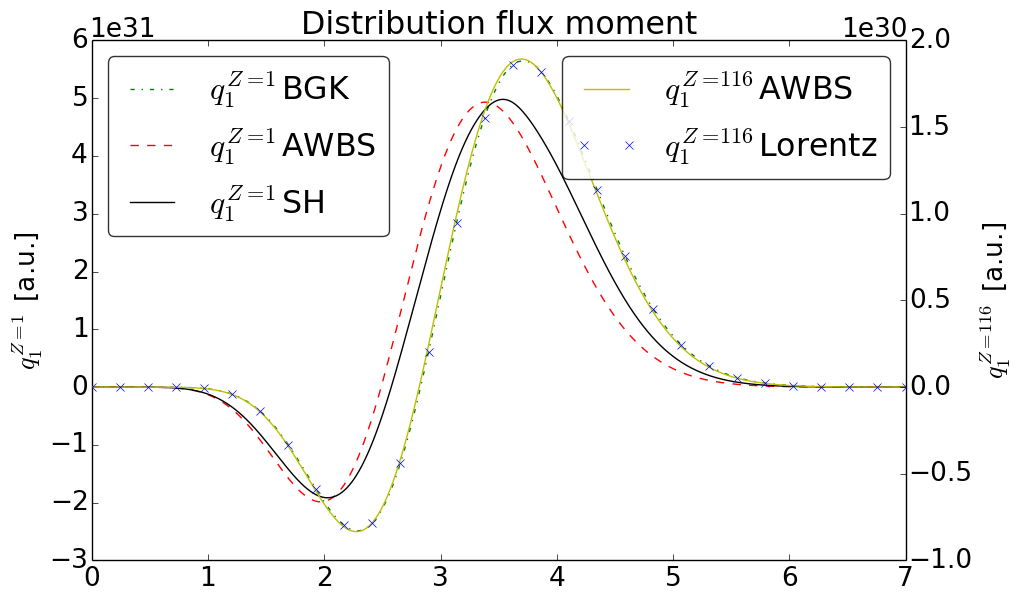
\includegraphics[width=0.5\textwidth]{q1s.png}
    \end{tabular}
  \caption{  
  The~flux velocity moment of the~anisotropic part of the~electron distribution 
  function in low $Z=1$ and high $Z=116$ plasmas in diffusive regime.}
  \end{center}
  \label{fig:q1s_summary}
\end{figure}

\begin{table}
\begin{center}
  \begin{tabular}{c|ccccc}
    \hline\hline\\
    %$\Zbar$ & $1$ & $2$ & $4$ & $16$ & $\infty$ \\\\
    & $\,\Zbar=1\,$ & $\,\Zbar=2\,$ & $\,\Zbar=4\,$ & $\,\Zbar=16\,$ & $\,\Zbar=116\,$ \\\\
    \hline\\
    $\bar{\Delta}\vect{q}_{AWBS}$ & 0.057 & 0.004 & 0.038 & 0.049 & 0.004 \\\\
    \hline\hline
  \end{tabular}
  \caption{
  Relative error $\bar{\Delta}\vect{q}_{AWBS} = 
  |\vect{q}_{AWBS} - \vect{q}_{SH}| / \vect{q}_{SH}$ of the~AWBS
  kinetic model equation \refeq{eq:AWBS_model} showing the~discrepancy 
  (maximum around 5$\%$) with respect to the~original solution of 
  the~heat flux given by numerical solution in Spitzer and Harm 
  \cite{SpitzerHarm_PR1953}.
  }
\end{center}
\label{tab:qAWBS}
\end{table}

